\documentclass[11pt,a4paper]{article}
\usepackage[utf8]{inputenc}
\usepackage[a4paper]{geometry}
\usepackage{amsthm}

\usepackage{float}
\usepackage{alltt} 
\usepackage{graphicx}
\usepackage{latexsym}
\usepackage{kpfonts} %font family
\usepackage{tikz}

\usepackage{xcolor}
\definecolor{bl}{RGB}{21, 101, 192}
\definecolor{grn}{RGB}{46, 125, 50}
\definecolor{rd}{RGB}{191, 54, 12}
\definecolor{prpl}{RGB}{156, 39, 176}

\usepackage[style=alphabetic, backend = bibtex]{biblatex}


% Standard number sets.
\newcommand{\N}{\mathbb{N}}
\newcommand{\Z}{\mathbb{Z}}
\newcommand{\Q}{\mathbb{Q}}
\newcommand{\R}{\mathbb{R}}
\newcommand{\C}{\mathbb{C}}

\newcommand{\bin}{\mathbb{F}_2}


% Fancy italic letters.
\newcommand{\A}{\mathcal{A}}
\newcommand{\B}{\mathcal{B}}

% Theorem environments.
\theoremstyle{plain}
\newtheorem{theorem}{Theorem}[section]
\newtheorem{proposition}[theorem]{Proposition}
\newtheorem{lemma}[theorem]{Lemma}
\newtheorem{corollary}[theorem]{Corollary}
\newtheorem*{question}{Question}

\theoremstyle{definition}
\newtheorem{definition}[theorem]{Definition}

\theoremstyle{remark}
\newtheorem{example}[theorem]{Example}
\newtheorem{remark}[theorem]{Remark}
\newtheorem{notation}[theorem]{Notation}


\title{Coding Theory and Sphere Packing}
\author{Andrei Nenciu}

\begin{document}
\maketitle

\section{Introduction}

\section{Noiseless Coding Theory}

\section{Error-Correcting Codes}

Consider a code \( c : \A 	\to \bin^n \) for some \( n \in N \). 
\begin{definition}
        The code \( c \) is said to be \( e \)-error detecting if, for any \( a \in \A \), changing at most \( e \) letters in \( c\left(a\right) \) does not give another code word.
\end{definition}

\begin{figure}[!h]
  \centering
  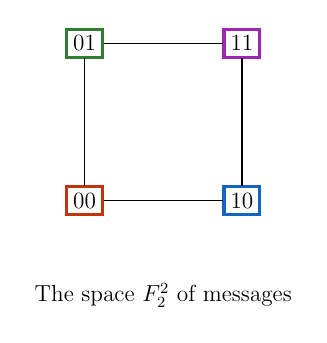
\begin{tikzpicture}[baseline, scale=2]
    \begin{scope}[yshift=-2.2 mm]
    \tikzset{font={\fontsize{12pt}{12}\selectfont}}
    \tikzstyle{every node}=[scale=0.7, rectangle, draw=black]
    \node [draw=rd, very thick]    (v0) at (0,0) {\( 00 \)};
    \node [draw=bl, very thick]    (v1) at (1,0) {\( 10 \)};
    \node [draw=grn, very thick]   (v2) at (0,1) {\( 01 \)};
    \node [draw=prpl, very thick]  (v3) at (1,1) {\( 11 \)};

    \draw (v0) -- (v1) -- (v3) -- (v2) -- (v0);
    \node[draw=white, below=2cm] at (current bounding box.base)
          {The space \( \bin^2 \) of messages};
    \end{scope}
  \end{tikzpicture}
  \hspace{2 cm}
  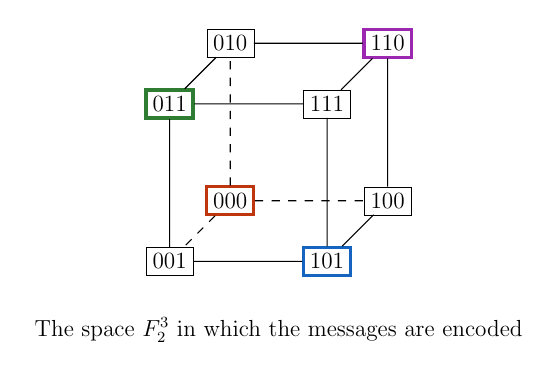
\begin{tikzpicture}[grow=right,baseline, scale=2]
    \tikzset{font={\fontsize{12pt}{12}\selectfont}}
    \tikzstyle{every node}=[scale=0.7, rectangle, draw=black]
    \node [draw=rd, very thick]   (v0) at (0,0,0) {\( 000 \)};
    \node [ultra thin]            (v1) at (1,0,0) {\( 100 \)};
    \node [ultra thin]            (v2) at (0,1,0) {\( 010 \)};
    \node [draw=prpl, very thick] (v3) at (1,1,0) {\( 110 \)};
    \node [ultra thin]            (v4) at (0,0,1) {\( 001 \)};
    \node [draw=bl, very thick]   (v5) at (1,0,1) {\( 101 \)};
    \node [draw=grn, very thick]  (v6) at (0,1,1) {\( 011 \)};
    \node [ultra thin]            (v7) at (1,1,1) {\( 111 \)};

    \draw (v4) -- (v5) -- (v7) -- (v6) -- (v4)
          (v5) -- (v1) -- (v3) -- (v7) -- (v5)
          (v6) -- (v2) -- (v3);
    \draw [dashed]
          (v0) -- (v1)
          (v0) -- (v2)
          (v0) -- (v4);
    \node[draw=white, below=2cm] at (current bounding box.base)
    {The space \( \bin^3 \) in which the messages are encoded};
  \end{tikzpicture}
\end{figure}

asfasdassdasad asdasdasd as das dasd asfasf sa fsdaf sa saf asf asfas dsa fasf saf asf asf sa dsagasdasd as sdasf asd asf asd a

\end{document}
